
\section{Purification Methods}
\label{sec: purification methods}

For the purposes removing the above-mentioned contaminants, hydrofluorination
has proven to be the most effective method of purifying molten fluoride salts
by ARE and MSRE scientists \cite{rev3}, \cite{rev21}. Hydrofluorination, in
these cases, is used as a blanket term to describe any process where a
substance is oxidized by a fluorinating agent then reduced by a hydrogenating
agent, producing \ch{HF} gas in the process. This method can be largely varied
using different fluorinating agents. Conceptually, if the redox potential is
the only property observed, pure fluorine gas would be the best for this
purpose. \ch{F2} was the first fluorinating agent used by the MSRE project for
their molten salt purification needs; however, pure fluorine gas proved to be
too corrosive to reactor vessels and was replaced \cite{rev21}. Varying the
hydrogenation agent is less flexible, as \ch{H2} gas has been used exclusively
due to its ease of access, lack of corrosive properties, and lack of toxicity.
\par

\subsection{\ch{HF}-\ch{H2} Sparging}
\label{sec: hf sparging}

\ch{HF-H2} sparging is by far the most accepted and well documented form of
purifying molten fluoride salt mixtures. This method consists of bubbling a
mixture of anhydrous \ch{HF} gas and \ch{H2} gas through the molten salt in a
sparge-tank-like reaction vessel. \par

\subsubsection{Chemistry}
\label{sec: hf chemistry}

\ch{HF-H2} sparging removes oxygen and sulfur by the reaction
mechanisms shown in

\Cref{eq: O2 to H2O,eq: OH to H2O,eq: SO4 to S2,eq: SO3 to S2,eq: S
to H2S} \cite{rev30}. \par

\begin{equation}
  \ch{O^{2-} + 2 HF <=> H2O + 2 F-} \label{eq: O2 to H2O} \\
\end{equation}

\begin{equation}
  \ch{OH^{-} + HF <=> H2O + F-} \label{eq: OH to H2O} \\
\end{equation}

\begin{equation}
  \ch{SO4^{2-} + 4 H2 <=> S^{-2} + 4 H2O} \label{eq: SO4 to S2} \\
\end{equation}

\begin{equation}
  \ch{SO3^{2-} + 3 H2 <=> S^{-2} + 3 H2O} \label{eq: SO3 to S2} \\
\end{equation}

\begin{equation}
  \ch{S^{2-} + 2 HF <=> H2S + 2F-} \label{eq: S to H2S} \\
\end{equation}

\ch{HF}, like all fluorinating agents, is corrosive to structural metals
(Me) through the reaction mechanism shown in \Cref{eq: metal
oxidation} \cite{rev30}. \par

\begin{equation}
  \ch{xMe + yHF <=> Me_xF_y + 0.5 yH2} \label{eq: metal oxidation}
\end{equation}

The corrosion of structural metals by HF adds metal contaminants to
the salt mix. The addition of \ch{H2} gas
suppresses this corrosion by not only acting as a reducing agent, but
also by pushing \cref{eq: SO4 to S2,eq: SO3 to S2} to the
right. Fluorination is however the rate limiting step of these
reactions, so the concentration of \ch{HF} in the
mix cannot be reduced too much without decreasing the reaction rate.
Because of this, an optimal mix
of \ch{HF} and \ch{H2} is required to balance reaction kinetics with vessel
corrosion. The optimal ratio by volume
of \ch{H2} to \ch{HF} was found to be roughly 10:1 \cite{rev21,rev30}. \par

\subsubsection{Kinetics}
\label{sec: hf kinetics}

Zong et al. found the optimal purification time, molten salt sparge
height, operating temperature, and
gas mixture flow rate for \SI{5}{\liter} of FLiNaK salt \cite{rev30}.
Assuming that
FLiBe is similar enough to FLiNaK
chemically and that the relationship between these values and molten
salt volume is sufficiently linear,
their data can be used to optimize the design of a reaction vessel
while maintaining roughly the same
purification time. The proper \ch{HF} effluent concentration at which to
halt purification can also be
determined. \par

\Cref{fig: oxygen vs time,fig: impurities vs time,fig: oxygen vs
  liquid height,fig:
oxygen vs temperature,fig: oxygen vs gas flowrate}
show their data.

\begin{figure}
  \centering
  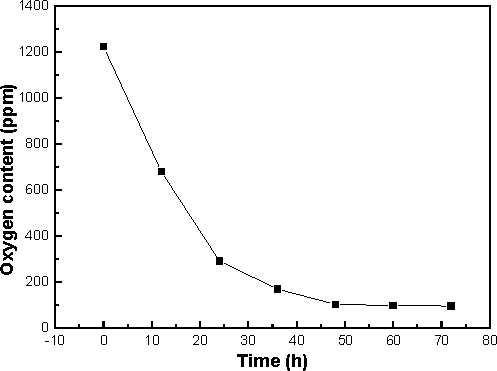
\includegraphics[width=0.6\textwidth]{./assets/review/figures/oxygen_vs_time.pdf}
  \caption{Oxygen content vs purification time for \SI{5}{\liter} of FLiNaK at
    a liquid height of \SI{0.9}{\meter} and \SI{650}{\celsius} at a gas
  flowrate of \SI{800}{\milli\liter\per\minute} \cite{rev30}}
  \label{fig: oxygen vs time}
\end{figure}

\begin{figure}
  \centering
  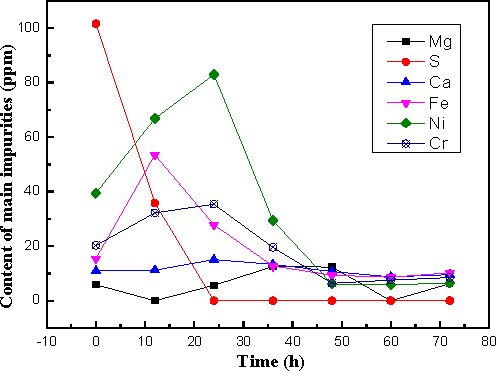
\includegraphics[width=0.6\textwidth]{./assets/review/figures/impurities_vs_time.pdf}
  \caption{Other impurity content vs purification time for \SI{5}{\liter} of
    FLiNaK at a liquid height of \SI{0.9}{\meter}, at \SI{650}{\celsius},
  at a gas flowrate of \SI{800}{\milli\liter\per\minute} \cite{rev30}}
  \label{fig: impurities vs time}
\end{figure}

\begin{figure}
  \centering
  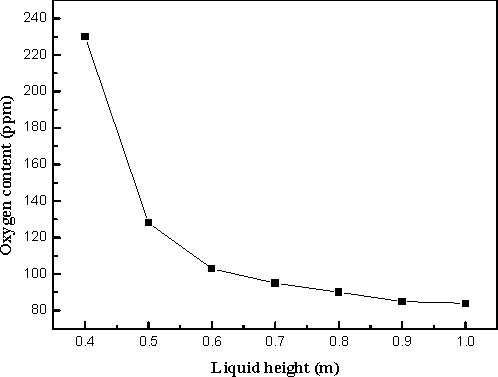
\includegraphics[width=0.6\textwidth]{./assets/review/figures/oxygen_vs_liquid_height.pdf}
  \caption{Oxygen content vs liquid height for \SI{5}{\liter} of FLiNaK run for
    \SI{48}{\hour} at \SI{650}{\celsius}, at a gas
  flowrate of \SI{800}{\milli\liter\per\minute} \cite{rev30}}
  \label{fig: oxygen vs liquid height}
\end{figure}

\begin{figure}
  \centering
  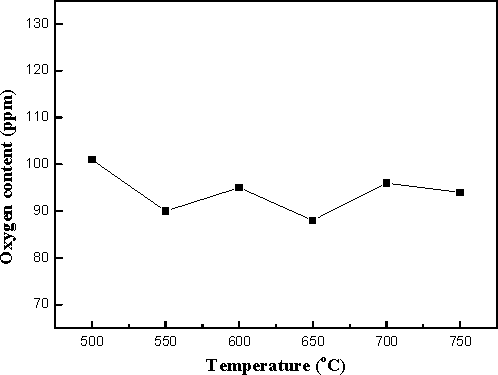
\includegraphics[width=0.6\textwidth]{./assets/review/figures/oxygen_vs_temperature.pdf}
  \caption{Oxygen content vs temperature for \SI{5}{\liter} of FLiNaK run for
    \SI{48}{\hour} at a liquid height of \SI{0.9}{\meter}, at a gas
  flowrate of \SI{800}{\milli\liter\per\minute} \cite{rev30}}
  \label{fig: oxygen vs temperature}
\end{figure}

\begin{figure}
  \centering
  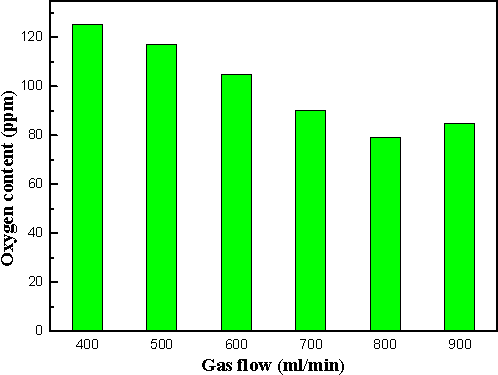
\includegraphics[width=0.6\textwidth]{./assets/review/figures/oxygen_vs_gas_flow_rate.pdf}
  \caption{Oxygen content vs gas flowrate for \SI{5}{\liter} of FLiNaK run for
    \SI{48}{\hour} at a liquid height of \SI{0.9}{\meter}, at
  \SI{650}{\celsius} \cite{rev30}}
  \label{fig: oxygen vs gas flowrate}
\end{figure}

\pagebreak

\Cref{fig: oxygen vs time,fig: impurities vs time}
shows that, all other factors being at their optimal state, there is
no appreciable change in
the concentrations of any of the impurities after roughly \SI{48}{\hour} of
hydrofluorination. This implies that
running for any longer than this time is pointless so long as the
system is optimized and gives a rough
maximum for hydrofluorination time. \Cref{fig: oxygen vs temperature}
shows that, all other
factors being at their optimal state,
the relationship between temperature and rate of oxide removal is
weak and relatively flat. This is likely
due to the increased gas residence time in cooler, more viscous salt
offsetting the drop in rate constant
caused by a decrease in temperature \cite{rev30}. \Cref{fig: oxygen
vs gas flowrate}
shows that, all other factors being at their optimal
state, there is an optimal gas flowrate to maximize the rate of oxide
removal, in this case, at \SI{800}{\milli\liter\per\minute}.
This flowrate likely allows for the optimal mix of HF and salt to
maximize reaction rate. How these
factors change with respect to the amount of salt being produced has
not been explored; however, it is
assumed to be linear. \par

\pagebreak

\subsubsection{Reagent Properties and Hazards}
\label{sec: hf reagent properties}

Anhydrous \ch{HF} is a clear, highly corrosive liquid/gas at room
temperature with a boiling point at \SI{19.5}{\celsius}.
\ch{HF} is also highly toxic (4 on NFPA diamond). It can
react with certain metals to release toxic and
flammable gases. When it contacts water, hydrofluoric acid is formed,
which is even more corrosive. Though not carcinogenic, it can cause
severe acid burns if contacted with skin and severe lung
inflammation and damage if inhaled. Because of its relatively high
boiling point, \ch{HF} can also present a clogging hazard in thin, unheated
lines. \cite{rev31} \par

\subsubsection{Reagent Costs}
\label{sec: hf reagent costs}

The upfront costs of HF are relatively low, but due to its relatively high
boiling point, trace heating on lines is necessary to minimize clogging
issues. Its high corrosivity also means that structural elements
will likely need to be replaced occasionally. \par

\subsection{\ch{NF3}-\ch{H2} Sparging/\ch{NF3} Baking}
\label{sec: nf3 sparging}

Although it has never been used before, \ch{NF3} has several theoretical
benefits over \ch{HF} as a fluorinating
agent, and thus may be a viable replacement. \ch{NF3} lack of use means
that there is no experimental data
to compare, so simulations by Scheele et all are the only source of
data. This also means that there is no
known preference for using \ch{NF3} with molten or solid salt. \par

\subsubsection{Chemistry and Thermodynamics}
\label{sec: nf3 chemistry and thermodynamics}

\Cref{eq: NF3 oxide fluorination,eq: NF3 hydroxide fluorination} show
the general reaction format for the reaction between \ch{NF3} and a component
salt oxide and hydroxide, respectively. \par

\begin{equation}
  \ch{3 y X_yO + 2 NF3 -> 3 y XF_{3 - y} + N2 + 1.5 O2 }
  \label{eq: NF3 oxide fluorination}
\end{equation}

\begin{equation}
  \ch{3 (3 - y) X (OH)_y + 2 NF3 -> 3 (3 - y) XF_y + N2 + 3 H2O + 1.5
  O2}
  \label{eq: NF3 hydroxide fluorination}
\end{equation}

As demonstrated by Scheele et all \cite{rev9} \ch{NF3} is a more
thermodynamically effective fluorinator than HF, as
it has a lower Gibbs free energy of reaction, for every major oxide
and hydroxide contaminant formed
with the component salts in FLiNaK and FLiBe. The use of \ch{NF3} also
introduces the possibility of removing
TRISO fuel components from molten salts as it can fluorinate \ch{C} and
\ch{UO2}, unlike \ch{HF}, a difference that
could prove useful for commercial uses as TRISO fuel continues to be
used more and more in other
reactor designs. TRISO particles could be dissolved in the salt as a
fuel source. This does imply that \ch{NF3}
can potentially be used for in-line purification. As stated
previously, no data has been found for the
general reaction between \ch{NF3} and sulfide, sulfate, or structural
metal contaminants. The Gibbs energies
of reaction between \ch{NF3} and the oxides of component salts, and
between \ch{HF} and the component salts
are shown in
\Cref{tab: beo nf3 beo hf table,tab:
  li2o nf3 li2o hf table,tab:
  beoh2 nf3 beoh2 hf table,tab:
  lioh nf3 lioh hf table,tab:
  na2o nf3 na2o hf table,tab:
  k2o nf3 k2o hf table,tab:
  naoh nf3 naoh hf table,tab:
koh nf3 koh hf table}.
\cite{rev31}
The Gibbs energies of the reaction
between \ch{NF3} with fuel components and
\ch{HF} with fuel components are shown in
\Cref{tab: uo2 nf3 uo2 hf table,tab:
  c nf3 c hf table,tab:
sic nf3 sic hf table}.
\cite{rev31} \par

\begin{table}
  \centering
  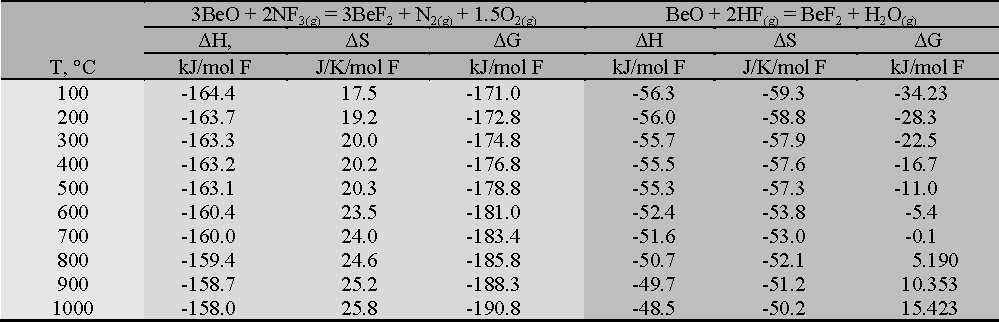
\includegraphics[width=0.6\textwidth]{./assets/review/figures/beo_nf3_beo_hf_table.pdf}
  \caption{\ch{NF3} + \ch{BeO} and \ch{HF} + \ch{BeO} Gibbs energies
  of reaction \cite{rev31}.}
  \label{tab: beo nf3 beo hf table}
\end{table}

\begin{table}
  \centering
  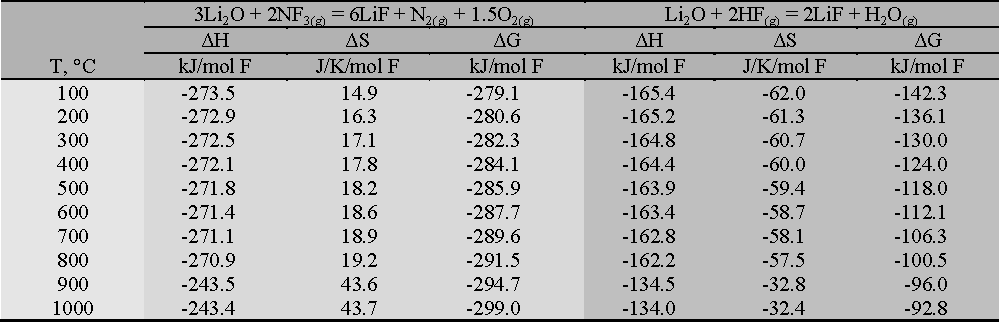
\includegraphics[width=0.6\textwidth]{./assets/review/figures/li2o_nf3_li2o_hf_table.pdf}
  \caption{\ch{NF3} + \ch{Li2O} and \ch{HF} + \ch{Li2O} Gibbs energies
  of reaction \cite{rev31}.}
  \label{tab: li2o nf3 li2o hf table}
\end{table}

\begin{table}
  \centering
  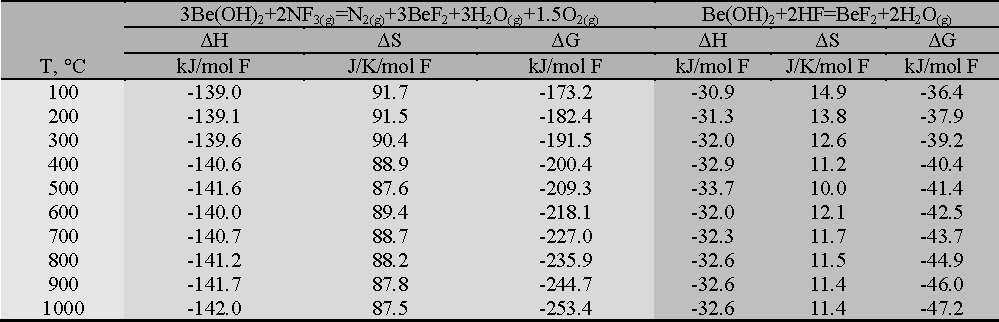
\includegraphics[width=0.6\textwidth]{./assets/review/figures/beoh2_nf3_beoh2_hf_table.pdf}
  \caption{\ch{NF3} + \ch{Be(OH)2} and \ch{HF} + \ch{Be(OH)2} Gibbs energies
  of reaction \cite{rev31}.}
  \label{tab: beoh2 nf3 beoh2 hf table}
\end{table}

\begin{table}
  \centering
  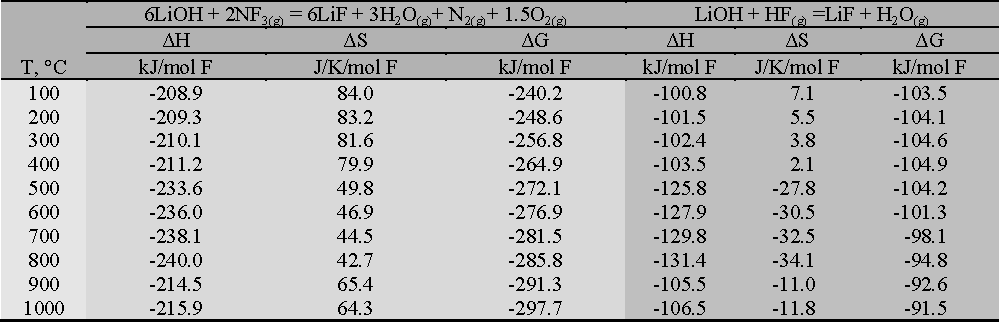
\includegraphics[width=0.6\textwidth]{./assets/review/figures/lioh_nf3_lioh_hf_table.pdf}
  \caption{\ch{NF3} + \ch{LiOH} and \ch{HF} + \ch{LiOH} Gibbs energies
  of reaction \cite{rev31}.}
  \label{tab: lioh nf3 lioh hf table}
\end{table}

\begin{table}
  \centering
  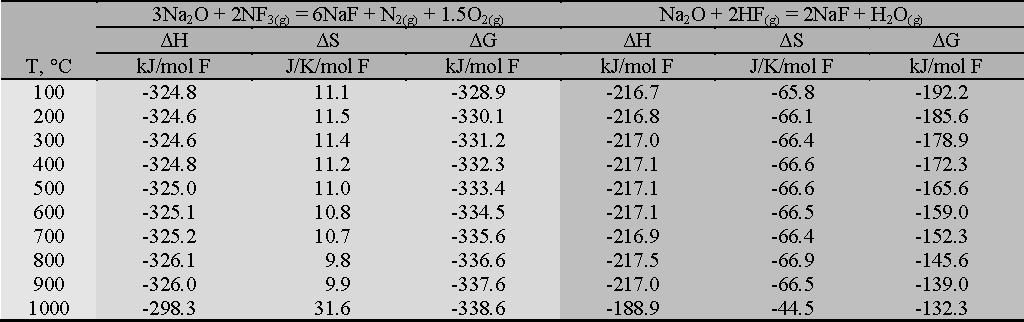
\includegraphics[width=0.6\textwidth]{./assets/review/figures/na2o_nf3_na2o_hf_table.pdf}
  \caption{\ch{NF3} + \ch{LiOH} and \ch{HF} + \ch{LiOH} Gibbs energies
  of reaction \cite{rev31}.}
  \label{tab: na2o nf3 na2o hf table}
\end{table}

\begin{table}
  \centering
  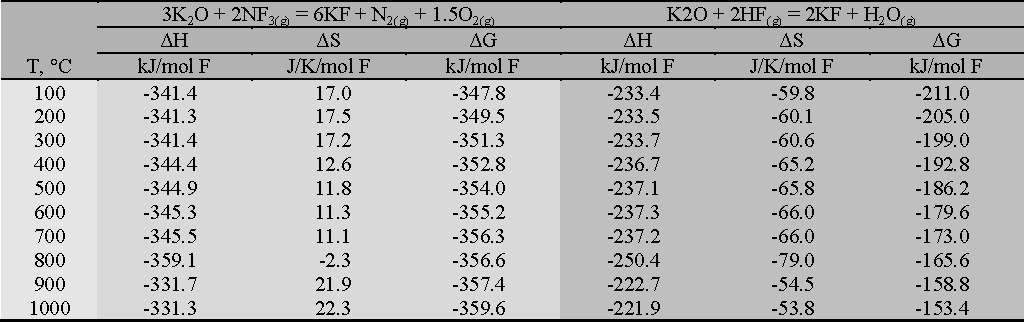
\includegraphics[width=0.6\textwidth]{./assets/review/figures/k2o_nf3_k2o_hf_table.pdf}
  \caption{\ch{NF3} + \ch{K2O} and \ch{HF} + \ch{K2O} Gibbs energies
  of reaction \cite{rev31}.}
  \label{tab: k2o nf3 k2o hf table}
\end{table}

\begin{table}
  \centering
  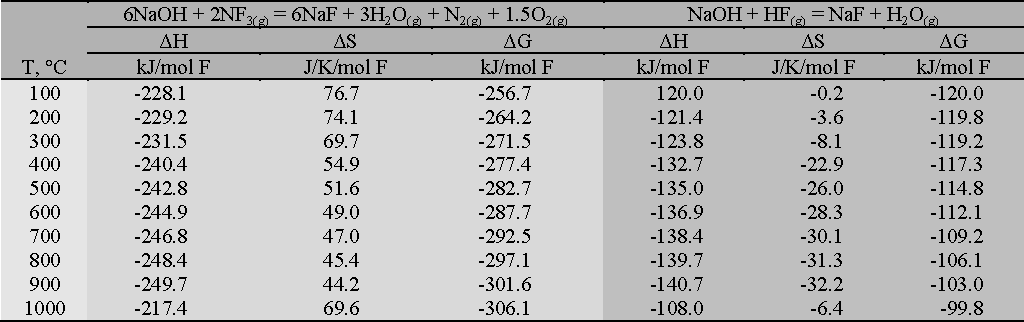
\includegraphics[width=0.6\textwidth]{./assets/review/figures/naoh_nf3_naoh_hf_table.pdf}
  \caption{\ch{NF3} + \ch{NaOH} and \ch{HF} + \ch{NaOH} Gibbs energies
  of reaction \cite{rev31}.}
  \label{tab: naoh nf3 naoh hf table}
\end{table}

\begin{table}
  \centering
  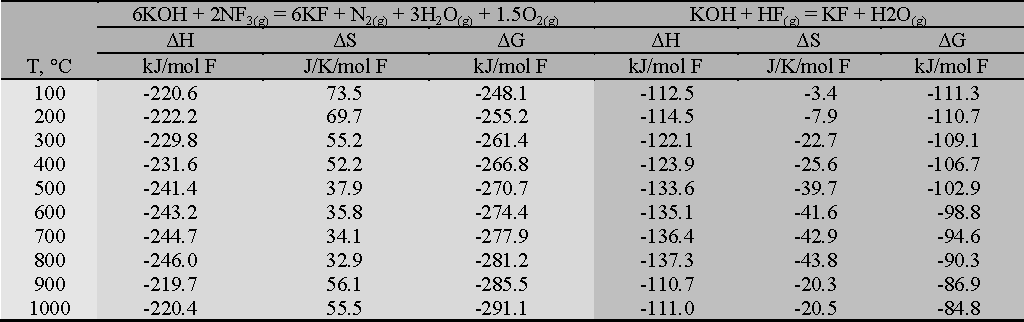
\includegraphics[width=0.6\textwidth]{./assets/review/figures/koh_nf3_koh_hf_table.pdf}
  \caption{\ch{NF3} + \ch{KOH} and \ch{HF} + \ch{KOH} Gibbs energies
  of reaction \cite{rev31}.}
  \label{tab: koh nf3 koh hf table}
\end{table}

\begin{table}
  \centering
  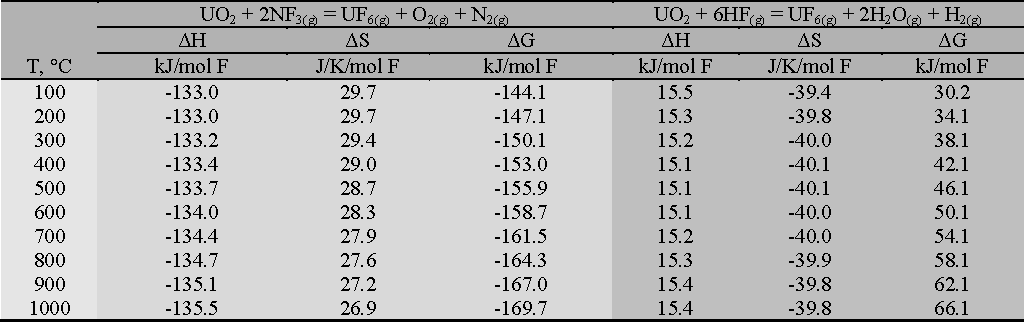
\includegraphics[width=0.6\textwidth]{./assets/review/figures/uo2_nf3_uo2_hf_table.pdf}
  \caption{\ch{NF3} + \ch{UO2} and \ch{HF} + \ch{UO2} Gibbs energies
  of reaction \cite{rev31}.}
  \label{tab: uo2 nf3 uo2 hf table}
\end{table}

\begin{table}
  \centering
  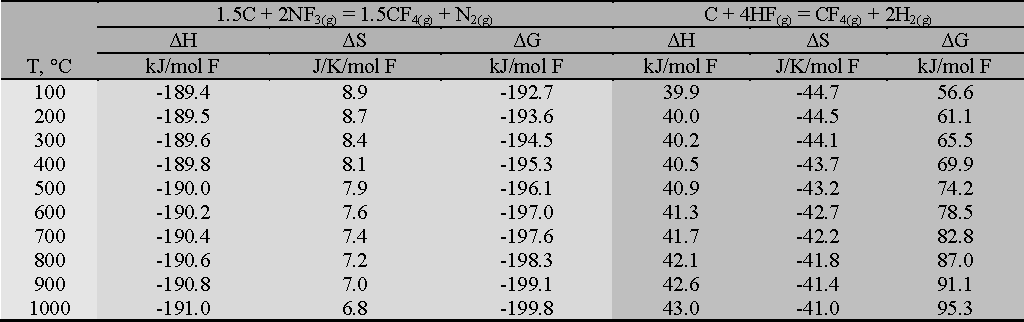
\includegraphics[width=0.6\textwidth]{./assets/review/figures/c_nf3_c_hf_table.pdf}
  \caption{\ch{NF3} + \ch{C} and \ch{HF} + \ch{C} Gibbs energies
  of reaction \cite{rev31}.}
  \label{tab: c nf3 c hf table}
\end{table}

\begin{table}
  \centering
  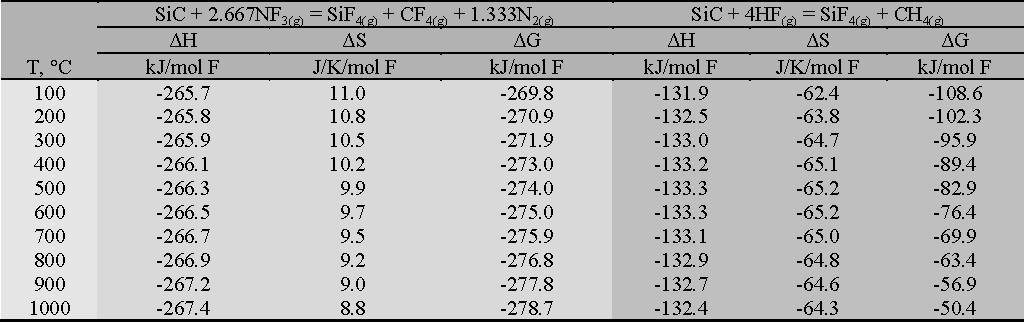
\includegraphics[width=0.6\textwidth]{./assets/review/figures/sic_nf3_sic_hf_table.pdf}
  \caption{\ch{NF3} + \ch{SiC} and \ch{HF} + \ch{SiC} Gibbs energies
  of reaction \cite{rev31}.}
  \label{tab: sic nf3 sic hf table}
\end{table}

\subsubsection{Kinetics}
\label{sec: kinetics}

No kinetic data is available for \ch{NF3} purification of molten salt;
however, its likely lower solubility in
molten salts when compared to HF presents an issue \cite{rev40}. The salt
viscosity needs to be optimized to
maximize residence time of the \ch{NF3} in the salt, while also still
allowing the \ch{NF3} to diffuse through the salt
without becoming trapped. \ch{NF3} also reacts in multistep processes
with some compounds which could lead to competing reactions \cite{rev31},
\cite{rev40}. An example of this is \ch{UO2} to \ch{UF6} by \ch{NF3}.
The \ch{U} will first change oxidation states from \ch{U^{4+}} to
\ch{U^{6+}} and form \ch{UO_2F_2} before turning into
\ch{UF6} \cite{rev31}. Changing oxidation states
requires higher temperatures than theorized and can be rate limiting.
Further study into the reactions between \ch{NF3} and the various compounds
present is necessary to determine which ones are a multistep process. \par

\subsubsection{Reagent Properties and Hazard}
\label{sec: nf3 hazards}

At lower temperatures, \ch{NF3} is a colorless gas, with oxidizing
properties similar to that of oxygen gas;
however, at temperatures exceeding \SI{400}{\celsius}, \ch{NF3} decomposes to
form fluorine radicals and behave more like fluorine gas \cite{rev31}. Because
of this, more noble alloys (such as Ni-200, Hastelloy-N, Monel 400, etc.)
are required for resisting the high corrosivity of \ch{NF3} at high
temperatures \cite{rev31}. \ch{NF3} is also considered a
significant greenhouse gas, as it has a global warming potential that
is \num{10800} times that of \ch{CO2} \cite{rev41}, and
will possibly become a regulated gas, requiring a recycling system to
be used \cite{rev31}. The physical
properties of \ch{NF3} are shown in \Cref{tab: nf3 properties}.
\cite{rev31} \par

Since the reactivity of \ch{NF3} is dependent on its temperature, it may
be preferable to bake the salts at a
lower temperature under a continuously flowing \ch{NF3} atmosphere. This
could potentially allow for a pure \ch{NF3} flow (as opposed to it being
diluted by hydrogen) but would be even more limited by the diffusion of
\ch{NF3} into the solid salt crystal structure. \par

\begin{table}
  \centering
  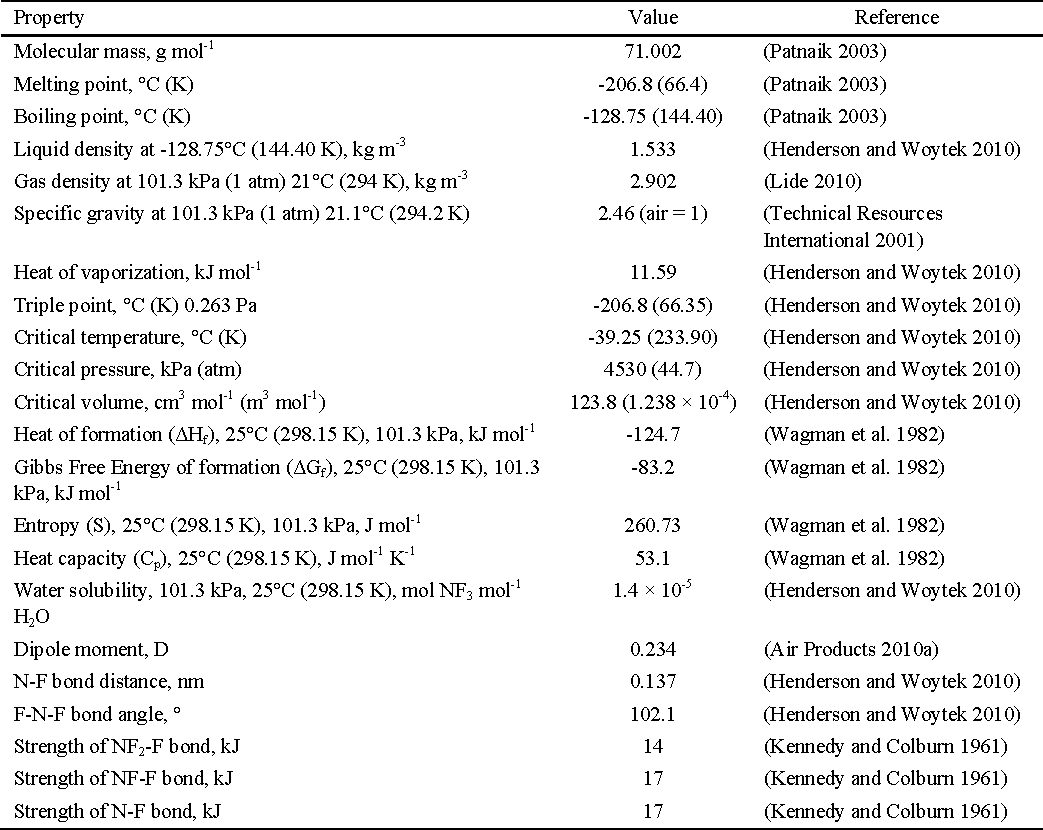
\includegraphics[width=0.6\textwidth]{./assets/review/figures/nf3_properties.pdf}
  \caption{Physical Properties of \ch{NF3} \cite{rev31}.}
  \label{tab: nf3 properties}
\end{table}

\subsubsection{Reagent Costs}
\label{sec: nf3 reagent costs}

For a lab grade purchase, \ch{NF3} will cost roughly 2.5-3 times as much as
\ch{HF} \cite{rev31}. Factoring in the possible cost of \ch{NF3} recovery
could further increase the cost of \ch{NF3} compared to that of \ch{HF};
however, because it is not as nearly corrosive, and is a gas at room
temperature, heat tracing and noble alloy piping and fittings are not
required to transport unheated \ch{NF3}. This could offset some of the
aforementioned costs compared to \ch{HF}. \par

\subsection{\ch{NF4HF2} Baking}
\label{sec: nf4hf2 baking}

Another available method for molten salt purification is \ch{NH4HF2}
baking. This
process involves the addition of high purity \ch{NH4HF2} to the frozen salt mix.
This mixture is then placed in a sealed container and brought up to
\qtyrange{600}{750}{\celsius} for \qtyrange{4}{24}{\hour} after which the
container is purged with an inert gas opened in an inert, dry atmosphere to
collect the purified salt \cite{rev42}.

\subsubsection{Chemistry}
\label{sec: nf4hf2 chemistry}

Above \SI{230}{\celsius}, \ch{NH4HF2} decomposes via the reaction shown in
\Cref{eq: nh4hf2 decomposition}. \cite{rev16} \par

\begin{equation}
  \ch{NH4HF2 -> NH3 + 2 HF} \label{eq: nh4hf2 decomposition}
\end{equation}

The \ch{NH3} produced in this reaction is inert relative to the salt and its
impurities; however, the \ch{HF} produced reacts in the same manner as what
was shown in \Cref{sec: nf3 chemistry and thermodynamics}. Since this method
relies on the produced \ch{HF} to react with the salt’s impurities, its
thermodynamics are the same as those for \ch{HF} shown in
\Cref{tab: beo nf3 beo hf table,tab:
  li2o nf3 li2o hf table,tab:
  beoh2 nf3 beoh2 hf table,tab:
  lioh nf3 lioh hf table,tab:
  na2o nf3 na2o hf table,tab:
  k2o nf3 k2o hf table,tab:
  naoh nf3 naoh hf table,tab:
  koh nf3 koh hf table,tab:
  uo2 nf3 uo2 hf table,tab:
  c nf3 c hf table,tab:
sic nf3 sic hf table}.
\par

This method will not purify the salt to the same extent as \ch{HF-H2} sparging.
\ch{HF-H2} sparging will bring the oxygen content down to $\sim\SI{80}{ppm}$
\cite{rev16,rev30},
while \ch{NH4HF2} baking will only bring oxygen content down to
$\sim\SI{200}{ppm}$ \cite{rev43},
with all other contaminants being at about equal concentrations for both
methods, besides sulfates which require a reaction with \ch{H2} as shown in
\Cref{eq: OH to H2O}
, meaning \ch{NH4HF2} baking will not remove this contaminant.
This shorter extent of purification could be explained by a number of
factors, but I believe that this is likely due to a lack of replenishment
of the \ch{HF} supply for the reaction. \par

\subsubsection{Kinetics}
\label{sec: nf4hf2 kinetics}

This method can reach \SI{200}{ppm} oxygen much faster than \ch{HF-H2}
sparging. While no studies into the kinetics of this method could be found,
a rough time of \SI{24}{\hour} was claimed to be sufficient to reach
\SI{200}{ppm} \cite{rev42}, \cite{rev43}. As shown in
\Cref{fig: oxygen vs time}, Zong et al. found that oxygen content was
around \SI{300}{ppm} after 24 hours for an optimized setup \cite{rev30}.
This may be due to increased contact between the \ch{HF} and oxygen
contaminants in \ch{NH4HF2} baking due to the
dispersal of \ch{NH4HF2} in the salt prior to heating as opposed to the
limited diffusion resulting from \ch{HF-H2} bubbling through the molten salt.
\par

\subsubsection{Reagent Properties and Hazards}
\label{sec: nf4hf2 hazards}

At room temperature, \ch{NH4HF2} takes the form of white crystals. This
allows it to be ground and mixed with salt eutectics at room temperature and
loaded into the reaction vessel all at once. While dangerous if ingested or
absorbed through the skin it presents no other harm in its solid state.
Primary hazards associated with this method are due to the \ch{HF} produced
upon heating of the \ch{NH4HF2}. Treatment of reaction effluent is the same
as \ch{HF-H2} sparging. Corrosion of the reaction vessel is less of a
concern with this method than with \ch{HF-H2} sparging due to the lower
concentration of \ch{HF} and the reduced exposure time. While less effective
than the aforementioned methods this method allows for a simpler reactor
setup and drastically decreased risk to health. \par

\subsection{Electrolytic Purification}
\label{sec: electrolytic purification}

A separate method of purification can be found in electrolysis of the
molten salt mix. This method does provide a couple of advantages versus
chemical purification. Electrolytic purification is both faster and less
wasteful than chemical purification and releases considerably less toxic
off gas. It is, however, less complete than chemical purification, with
oxide concentrations only going as low as $\sim\SI{200}{ppm}$ with just
electrolysis \cite{rev44}. It also cannot remove all metal impurities
from the salt. \ch{Cr} in particular will remain in solution as \ch{CrF2}.
\par

As stated previously, the first experiments for using electrolysis to
purify molten fluoride salt were done as part of the ARE in late 1954
\cite{rev5}. They used an electrolytic cell containing a graphite rod
anode and a nickel mesh cathode to help drop the fluorination potential
of salts by reducing dissolved metal fluorides to their metallic form
and releasing fluorine gas, which would be converted to hydrogen
fluoride by reacting with a padding hydrogen blanket above the salt
\cite{rev5}. \Cref{eq: metal electro reduction,eq: hydrogen}
show the reaction pathway. This method was introduced as a faster way of
reducing the fluorination potential of the salt compared to pure hydrogen
sparging and showed promise but was never introduced into the production
process and quickly dropped for unspecified reasons. This could be due to
issues found with the method, a lack of want to modify existing purification
equipment at the time, or advantages associated with using reducing agents
to help accelerate fluoride reduction instead. \par

\begin{equation}
  \ch{MeF2_{(eq)} ->[electrolysis] Me_{(s)} + F2_{(g)}}
  \label{eq: metal electro reduction}
\end{equation}

\begin{equation}
  \ch{H2 + F2 -> 2 HF}
  \label{eq: hydrogen}
\end{equation}

Experiments by Wang et al. have re-opened the possibility of using
electrolytic means to purify molten salts \cite{rev44}. The results of
their experiments showed that a \ch{C}, \ch{Ni} electrode could be used to
reduce the oxide concentration in an unspecified amount of FLiNaK down from
\SI{1000}{ppm} to around \SI{200}{ppm} in a matter of \SI{20}{\hour}hr.
They also showed a reduction in several metal contaminants. \par

Very recently, a molten fluoride salt electrolytic purification experiment
was performed by Zuo et al. \cite{rev27}. Their experiment focused on
improving the performance of electrolytical purification methods through
the addition of a continuous hydrogen sparge to the electrolytic setup.
Their cell design is shown in
\Cref{fig: electrocell}
nickel tube of flowing hydrogen gas is lowered into a nickel crucible filled
with molten salt, and electrodes are connected to the tube and crucible,
effectively creating a \ch{H^+}/\ch{H2}, \ch{Ni} electrode instead of the
\ch{C}, \ch{Ni} electrode used during the ARE experiments. A nickel foil
was used to increase the surface area of the nickel electrode. This setup
was able to get an unspecified amount of FLiNaK salt down below
\SI{100}{ppm} of oxygen contaminants in just a couple of hours.
The hydrogen sparge would also cause Ni and Fe impurities to be somewhat
reduced out of solution. Issues with scaling up this process were brought
up, namely that the current through the salt is low, presenting a
potential size limit for a given voltage. \par

\begin{figure}
  \centering
  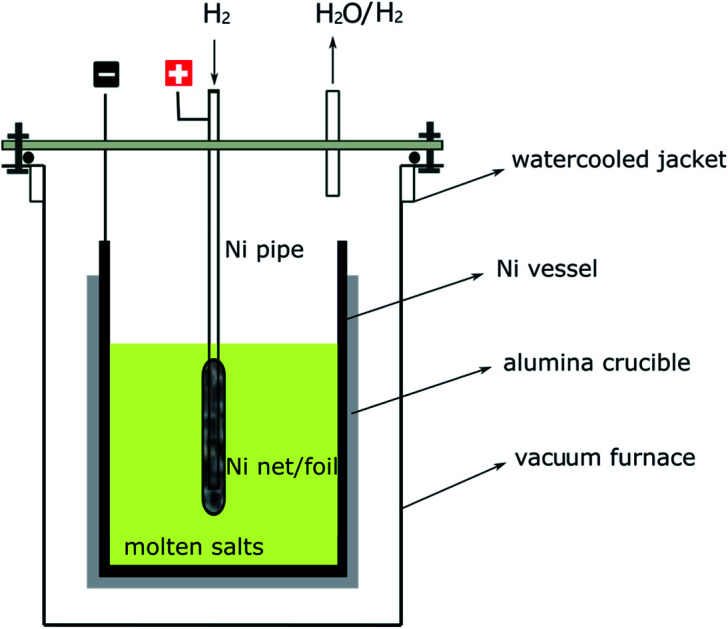
\includegraphics[width=0.5\textwidth]{./assets/review/figures/electrocell.jpg}
  \caption{Molten salt electrolytic purification vessel design used
  by Zuo el al.}
  \label{fig: electrocell}
\end{figure}

Although no prior studies had been performed to determine the effectiveness
of electrolytic purification of a fluoride salt, there had been studies
undertaken and methods developed for purification in some chloride salts
\cite{rev32,rev45,rev46}. Ding et all have produced complex, proven
electrolytic cells for the monitoring and purification of \ch{Mg} bearing
chloride salts \cite{rev45}. A diagram of the purification setup is shown in
\Cref{fig: chloride electrocell}. By using a sacrificial \ch{Mg} anode
and a \ch{W} cathode, hydroxides in the melt were reduced to \ch{MgO},
and the concentration of corrosive hydroxides in the melt was reduced by
\SI{93}{\percent} in a matter of a few minutes. The kinetics of this type
of electrochemical cell are limited by the buildup of a passivation layer
on the cathode. This effect can be mitigated by substituting the \ch{W}
used in the cathode for \ch{Mg} and using alternating voltage to
periodically swap the direction of electron flow \cite{rev46}.
\par

\begin{figure}
  \centering
  \includegraphics[width=0.6\textwidth]{./assets/review/figures/chloride
  electrocell.pdf}
  \caption{Schematic of assumed reactions and observed phenomena on the
    \ch{W}-cathode and \ch{Mg} anode in
    the electrochemical purification
  using pulsed over-potential.}
  \label{fig: chloride electrocell}
\end{figure}

The limited amount of research into this area presents a challenge and an
opportunity. From the beginning, electrolytic purification setups have
always been modifications to existing hydrofluorination setups so modifying
existing designs would likely not be difficult. Plenty of research exists
for using electrolytic salts to purify other metals, but little exists for
purifying the salts themselves. \par
